\section{Umsetzung des realen Clusters}\label{sec:aufbauCluster}

\subsection{Hadoop-Benchmark}\label{sec:hadoopBenchmark}

\citeauthor{zhang2016} haben im Rahmen ihrer gesamten Forschungsarbeit die Plattform Hadoop-Benchmark entwickelt und auf Github zur Verfügung gestellt\footnote{\url{https://github.com/Spirals-Team/hadoop-benchmark}}. Die Plattform ist in mehrere Szenarien unterteilt, darunter ein Hadoop 2.7.1 ohne Änderungen und ein Szenario mit der Selfbalancing-Komponente. Hadoop-Benchmark basiert auf der Software \emph{Docker}\footnote{\url{https://www.docker.com/}} und dem dazugehörigen Tool \emph{Docker Machine}, um damit einfach und schnell ein Hadoop-Cluster aufbauen zu können. Mit \emph{Graphite}\footnote{\url{https://graphiteapp.org/}} ist zudem ein Monitoring-Tool enthalten, mit dem die Performance des Clusters überwacht und analysiert werden kann.

\begin{figure}
    \centering
    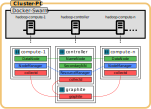
\includegraphics[width=.8\columnwidth]{./images/hadoopBenchmarkArch.png}
    \caption[High-Level-Architektur von Hadoop-Benchmark]{High-Level-Architektur von Hadoop-Benchmark \cite{abb:hadoopBenchmarkArch}}
    \label{fig:hadoopBenchmarkArchitecture}
\end{figure}

Mithilfe von Docker Machine können spezielle Virtuelle Maschinen erstellt werden, die direkt für den Einsatz mit Docker ausgestattet sind. Auf jeder dieser VMs können dadurch direkt ein oder mehrere Docker-Container gestartet werden, welche letztlich das Hadoop-Cluster bilden. Jeder Container enthält, neben dem Hadoop-Controller bzw. -Node, das Tool \emph{collectd}\footnote{\url{https://collectd.org/}}, was das Monitoring des Hadoop-Nodes auf Systemebene übernimmt und die Daten an den Graphite-Container auf der Controller-Machine übermittelt. Es ist dabei möglich, eine beliebige Anzahl an Nodes zu nutzen. Auch ist es möglich, den VMs einen beliebig großen Arbeitsspeicher zur Verfügung zu stellen.

Die Plattform Hadoop-Benchmark enthält auch die bereits in \autoref{sec:lastprofilerstellung} erwähnten Benchmarks Mapreduce Examples, HiBench und SWIM. Sie werden ebenfalls als jeweils eigene Docker-Container gestartet und so an das Cluster übermittelt.

\subsection{Genutztes Cluster in der Fallstudie}\label{sec:clusterFallstudie}

Als reales Hadoop-Cluster für diese Fallstudie soll nun ebenfalls die Plattform Hadoop-Benchmark zum Einsatz kommen. Da das Cluster eine Linux-Umgebung benötigt, wird dazu ein eigener PC genutzt, auf dem Ubuntu 16.04 LTS installiert ist. Da \sS das .NET-Framework, und damit Windows, benötigt, wird dafür ein eigener PC verwendet. Im konkreten Versuchsaufbau wird für Windows ebenfalls eine VM genutzt, welche auf dem anderen PC als das Cluster läuft. Die genauen Spezifikationen der PCs und der Windows-VM sind in \autoref{fig:pcSpecs} aufgelistet.

Auf dem Cluster-PC nutzt Docker-Machine zur Erstellung, Verwaltung und Ausführung der VMs die Treiber von VirtualBox 5.2\footnote{\url{https://www.virtualbox.org/}}. Für das Cluster werden 4 Nodes, der Controller sowie eine Consul-VM zur Verwaltung der Netzwerkverbindungen zwischen den VMs erstellt. Jede der vier Nodes und der Controller erhalten jeweils 2 GB RAM, der Consul erhält 512 MB.

\begin{figure}
    \centering
    \begin{tabular}{|c|c|c|c|}
    	\hline
    	     \textbf{}      & \textbf{Cluster-PC} & \textbf{VM-PC} &     \textbf{VM}      \\ \hline\hline
    	   \textbf{CPU}     &    Intel Core i5    & Intel Core i5  &       2 Cores        \\ \hline
    	   \textbf{RAM}     &        16 GB        &     16 GB      &         6 GB         \\ \hline
    	\textbf{Festplatte} &     500 GB HDD      &   128 GB SSD   &  $\leq$ 100 GB VHD   \\ \hline
    	    \textbf{OS}     &  Ubuntu 16.04 LTS   & Kubuntu 16.10  & Windows 10 1709 Edu. \\ \hline
    \end{tabular}
    \caption{Spezifikationen der verwendeten PCs und VM}
    \label{fig:pcSpecs}
\end{figure}

In keinem Szenario der Plattform Hadoop-Benchmark wird standardmäßig der Timeline-Server von Hadoop gestartet. Daher wurde basierend auf dem Selfbalancing-Szenario ein neues Szenario erstellt, bei dem der Timeline-Server gestartet wird. Dadurch ist einerseits die Selfbalancing-Komponente von \citeauthor{zhang2016} aktiv und andererseits besteht die Möglichkeit, mithilfe des Timeline-Servers das Monitoring des Clusters durchzuführen.
%TODO: Link zum angepassten Hadoop-Benchmark?

% Hilfsscript zur einfachen Verwaltung!